\documentclass[a4paper, 12pt]{article}
\usepackage[utf8]{inputenc}
\usepackage[T1]{fontenc}
\usepackage[french]{babel}
\usepackage{graphicx}
\usepackage{amsmath}
\usepackage{amssymb}
\usepackage{hyperref}
\usepackage{lmodern}
\pagestyle{headings}
\setlength{\parindent}{0pt}

\title{Compte rendu - Projet programmation fonctionnelle}
\author{Dorine Descamps et Marwan Ait Addi}
\date{\today}

\begin{document}

\maketitle
\tableofcontents
\newpage

Afin de faire un choix de liste cohérent, nous avons testé le temps que mettaient nos fonctions à trier des listes en faisant changer plusieurs variables. L'ordre étant une variable possible nous gardons l'ordre croissant pour tous les autres tests. Nous arrondirons les temps en fonctions des résultats, l'unité étant la seconde.

\section{Expérience}

\subsection{Comparaison du temps des fonctions de tri en augmentant la taille des listes}

Nous nous plaçons dans une fourchette d'entier de 0 à 100 pour le choix des éléments de la liste et augmentons la taille de la liste.
\begin{center}
\begin{tabular}{|c|c|c|c|c|c|c|}
\hline 
nombre d'éléments de la liste & 10 & 100 & 1000 & 10 000 & 25 000 & 50 000 \\ 
\hline 
temps tri$\_$partition$\_$fusion & 0 & 0 & 0.003 & 0.043 & 0.13 & 0.29 \\ 
\hline 
temps tri$\_$pivot & 0 & 0 & 0.002 & 0.051 & 0.36 & 1.83 \\ 
\hline 
temps tri$\_$bulle & 0 & 0.002 & 0.2 & 28.34 & \multicolumn{2}{c|}{cf remarque} \\ 
\hline
\end{tabular}
\end{center} 

Remarque : Nous ne traitons plus la fonction tri à bulle pour les listes de 25 000 et 50 000 éléments,2 sachant que les temps seront énormes (compté en minute voire dizaine de minutes). \\

Plus visuellement : 
\begin{center}
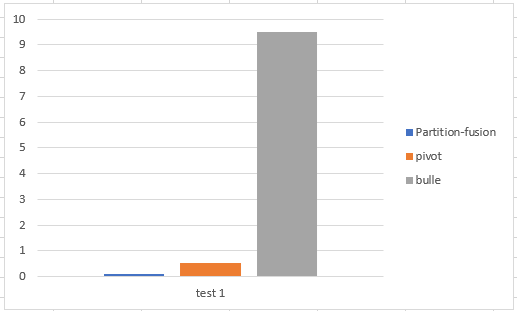
\includegraphics[scale=1]{graphique/test1.PNG} 
\end{center}

Il apparaît déjà que le tri à bulle est la manière de trier la moins optimisé sur de grande liste mais aussi que la fonction la plus rapide semble être le tri par partition-fusion.

\subsection{Comparaison du temps des fonctions de tri en augmentant la fourchette d'éléments possible}

Cette fois-ci, nous gardons la taille de la liste constante à 1000 éléments et augmentons la fourchette d'entier possible. 
\begin{center}
\begin{tabular}{|c|c|c|c|c|}
\hline 
fourchette d'éléments de la liste & 50 & 500 & 5000 & 10 000 \\ 
\hline 
temps tri$\_$partition$\_$fusion & 0.003 & 0.003 & 0.003& 0.006 \\ 
\hline 
temps tri$\_$pivot & 0.002 & 0.002 & 0.002 & 0.004\\ 
\hline 
temps tri$\_$bulle & 0.22 & 0.25 & 0.23 & 0.25 \\ 
\hline 
\end{tabular} 
\end{center}

Plus visuellement : 
\begin{center}
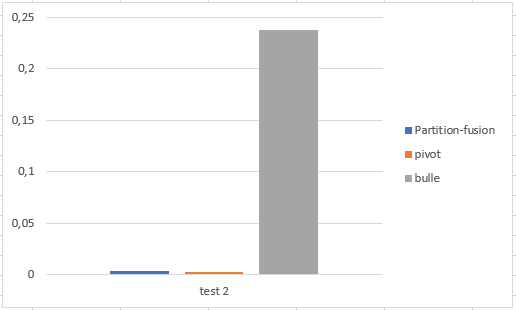
\includegraphics[scale=1]{graphique/test2.PNG} 
\end{center}

Nous pouvons remarqué que la fourchette d'éléments n'est pas une variable très important, les résultats sont relativement stables même si le pivot est le plus rapide.

\subsection{Comparaison du temps des fonctions de tri en fonction de l'ordre} 

Pour cette partie nous prenons une liste de 1000 éléments compris entre 0 et 5000 et changeons l'ordre de tri. 
\begin{center}
\begin{tabular}{|c|c|c|c|c|}
\hline 
ordre & < & > & <= & >= \\ 
\hline 
temps tri$\_$partition$\_$fusion & 0.004 & 0.003 &0.0030 & 0.002 \\ 
\hline 
temps tri$\_$pivot & 0.002 & 0.002 & 0.0020 & 0.001\\ 
\hline 
temps tri$\_$bulle & 0.23 & 0.21 & 0.229 & 0.23 \\ 
\hline  
\end{tabular}
\end{center} 
\newpage

Plus visuellement : 
\begin{center}
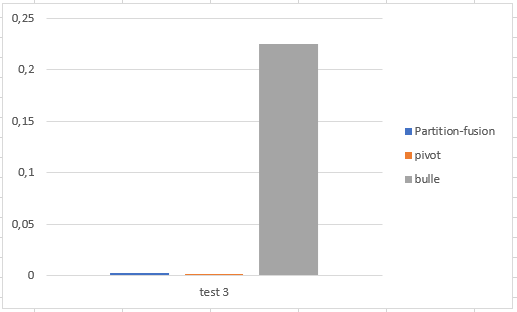
\includegraphics[scale=1]{graphique/test3.PNG} 
\end{center}

Là aussi, nous remarquons que l'ordre n'impacte pas beaucoup le temps de résolution, les résultats restent plutôt constants et le tri par pivot est toujours plus rapide.  

\subsection{Comparaison du temps des fonctions de tri en fonction du nombre de doublons}

Ici, nous utilisons des listes de 100 éléments entre 0 et 100 modifiés à la main pour avoir la quantité de doublons voulue.
\begin{center}
\begin{tabular}{|c|c|c|c|c|}
\hline 
Quantité de doublons & 100$\%$ & environ 50$\%$ & 25$\%$ & aucun \\ 
\hline 
temps tri$\_$partition$\_$fusion & 0.001 & 0 &0.001 & 0.001 \\ 
\hline 
temps tri$\_$pivot & 0.08 & 0 & 0.001 & 0\\ 
\hline 
temps tri$\_$bulle & 0 & 0.004 & 0.005 & 0.001 \\ 
\hline  
\end{tabular}
\end{center}
\newpage

Plus visuellement : 
\begin{center}
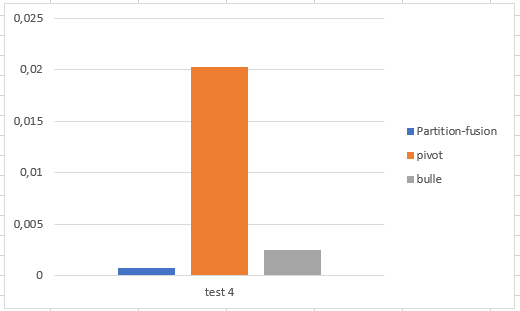
\includegraphics[scale=1]{graphique/test4.PNG} 
\end{center}

Les chiffres de cette expérience ne donnent pas de résultats flagrants, si ce n'est que le tri à bulle est toujours à la traine.  
  
\subsection{Comparaison du temps des fonctions de tri avec des listes déjà triées}

Pour ces tests nous utilisons des listes déjà triées de 1000 éléments entre 0 et 1000 et nous étudions le réaction des fonctions en fonction de l'ordre donné en paramètre.

\subsubsection{Liste trié dans l'ordre croissant stricte (<)}

\begin{center}
\begin{tabular}{|c|c|c|c|c|}
\hline 
ordre & < & > & <= & >= \\ 
\hline 
temps tri$\_$partition$\_$fusion & 0.002 & 0.003 &0.007 & 0.003 \\ 
\hline 
temps tri$\_$pivot & 0.08 & 0.11 & 0.07 & 0.1\\ 
\hline 
temps tri$\_$bulle & 0 & 0.22 & 0 & 0.24 \\ 
\hline  
\end{tabular}
\end{center} 

\subsubsection{Liste trié dans l'ordre décroissant stricte (>)}

\begin{center}
\begin{tabular}{|c|c|c|c|c|}
\hline 
ordre & < & > & <= & >= \\ 
\hline 
temps tri$\_$partition$\_$fusion & 0.002 & 0.003 &0.003 & 0.003 \\ 
\hline 
temps tri$\_$pivot & 0.07 & 0.09 & 0.07 & 0.07\\ 
\hline 
temps tri$\_$bulle & 0.03 & 0 & 0.23 & 0 \\ 
\hline  
\end{tabular} 
\end{center}

\subsubsection{Liste trié dans l'ordre croissant non stricte (<=)}

\begin{center}
\begin{tabular}{|c|c|c|c|c|}
\hline 
ordre & < & > & <= & >= \\ 
\hline 
temps tri$\_$partition$\_$fusion & 0.002 & 0.002 &0.003 & 0.006 \\ 
\hline 
temps tri$\_$pivot & 0.09 & 0.09 & 0.07 & 0.1\\ 
\hline 
temps tri$\_$bulle & 0 & 0.001 & 0 & 0.25 \\ 
\hline 
\end{tabular}
\end{center} 

\subsubsection{Liste trié dans l'ordre décroissant non stricte (>=)}

\begin{center}
\begin{tabular}{|c|c|c|c|c|}
\hline 
ordre & < & > & <= & >= \\ 
\hline 
temps tri$\_$partition$\_$fusion & 0.006 & 0.006 &0.003 & 0.002 \\ 
\hline 
temps tri$\_$pivot & 0.12 & 0.07 & 0.067 & 0.08\\ 
\hline 
temps tri$\_$bulle & 0.2 & 0.24 & 0.26 & 0 \\ 
\hline  
\end{tabular}
\end{center} 

Plus visuellement : 
\begin{center}
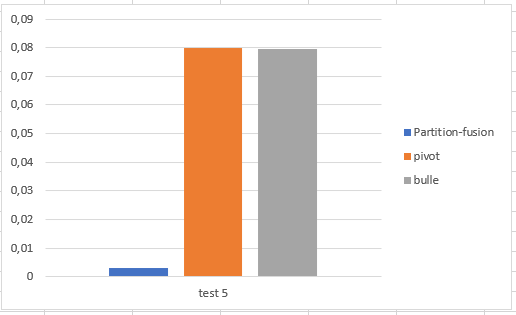
\includegraphics[scale=1]{graphique/test5.PNG} 
\end{center}

Il apparaît que la fonction bulle est la plus efficace pour trié une liste déjà trié dans le même ordre, ce qui est tout a fait logique mais pour le reste c'est la fonction tri partition fusion qui est la plus rapide. \newpage

\section{Résultats}

En faisant la moyenne de tous les tests on obtient donc : 
\begin{center}
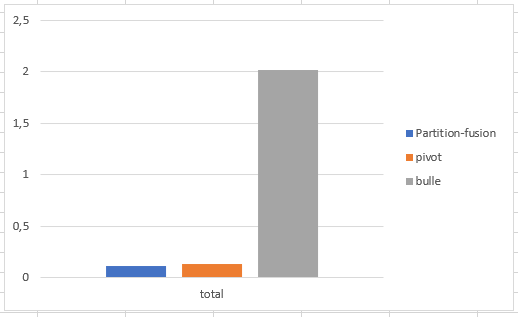
\includegraphics[scale=1]{graphique/final.PNG} 
\end{center}

Il apparaît clairement que le tri a bulle n'est pas optimisé, mais le tri par partition fusion reste légèrement plus rapide que le tri pivot, c'est donc le tri par partition-fusion que nous garderons pour le module de tri des listes.

\end{document}